\textbf{COLUNI 2024 -- Questão 23}\par\medskip Observe as figuras abaixo:

\noindent
\begin{minipage}[t]{0.48\linewidth}
\begin{center}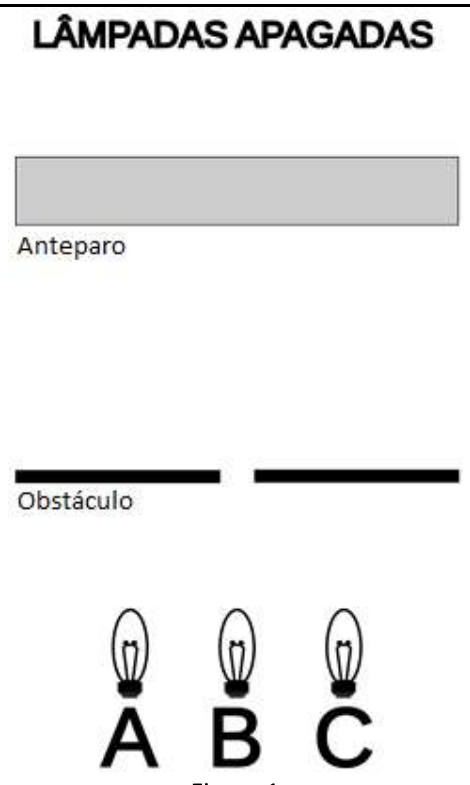
\includegraphics[width=\linewidth,trim=0 8pt 0 0,clip]{static/simulados/coluni/figuras/2024/questao-23/figura-1.png}\\Figura 1\end{center}
\end{minipage}\hfill
\begin{minipage}[t]{0.48\linewidth}
\begin{center}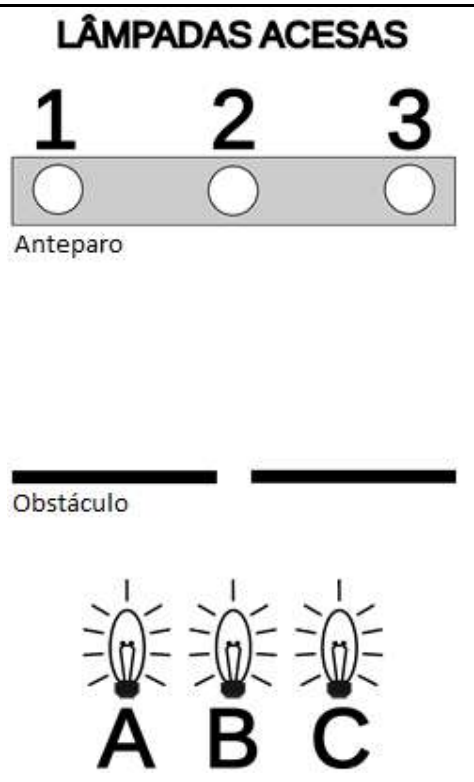
\includegraphics[width=\linewidth,trim=0 8pt 0 0,clip]{static/simulados/coluni/figuras/2024/questao-23/figura-2.png}\\Figura 2\end{center}
\end{minipage}

A figura 1 ilustra um experimento no qual três pequenas lâmpadas A, B e C, são posicionadas em frente a um obstáculo com um pequeno orifício central. Após o obstáculo, há um anteparo. Ao acender as três lâmpadas, observa-se que as regiões 1, 2 e 3 do anteparo são iluminadas, conforme ilustra a Figura 2.

Considere as afirmações sobre o experimento.

I. Acendendo a lâmpada C, apenas a região 3 do anteparo será iluminada.

II. Acendendo as lâmpadas B e C, apenas as regiões 1 e 2 do anteparo serão iluminadas.

III. Acendendo as lâmpadas A e B, apenas as regiões 1 e 2 do anteparo serão iluminadas.

IV. Acendendo as lâmpadas B e C, apenas as regiões 2 e 3 do anteparo serão iluminadas.

Está CORRETO o que se afirma apenas em:
\begin{enumerate}
\item I.
\item II.
\item III e IV.
\item I, III e IV.
\end{enumerate}
